\chapter{Enhancing ASEAN connectivity through Space and Geospatial Technology} \label{enhancing}

\tab Space and Geospatial Technology (SGT) is an intelligence technology enabling the global monitoring of a wide range of parameters such as the distribution of facilities and buildings, the movements of cars, ships, aircrafts, and people, environmental change, or post-disaster economic development processes. While geospatial technology was originally developed for military and security use, it has been,in recent years, quickly advanced towards an utilization as a \textbf{general civil technology}. It is now widely applied in the field of public services (e.g. disaster response, social infrastructure management, traffic management), business support (e.g. marketing), and personal mobility services (e.g. navigation). The extensive use of low-cost and high-performance mobile devices --- such as smart-phones --- has further accelerated its popularization all over the world. Later, the development of \textit{Internet of Things} (IoT) and \textit{Artificial Intelligence} (AI) technologies enabled researchers to conduct \textbf{deeper analyses, and quicker and broader information collection}. In this regard, geospatial technology has been expected to expand much further its utilization and development in the future.

\vspace{0.4 cm}

This chapter will be organized as follows:

\begin{enumerate}

\item Define and introduce generally the potential of SGT in various fields.

\item Present the original application of SGT (disaster management) and its wider potential for economic strengthening.

\item Finally, develop more concrete consideration on the use of SGT and data sharing to advance towards data driven ASEAN.

\end{enumerate}


\section{The immense potential of Space and Geospatial Technology}

\tab This section aims at introducing the concept of SGT and at briefly presenting general applications of SGT.

\subsection{What is SGT?} \label{wi_sgt}

The rise of intelligence technologies resulted in the development of three different technological areas of \textbf{space infrastructure}: 

\begin{itemize}

\item \textbf{Satellite-based earth observation technology}, monitoring occurrences all over the world.

\item \textbf{Positioning technology}, measuring and tracking precise positions in real time.

\item And \textbf{Communication technology} to connect almost instantly every single part of the world.

\end{itemize}

The most important application of space infrastructure (observation, positioning and communication) is what is called \textbf{Geospatial Technology}. Geospatial technology can be seen as a global information technology, providing services anywhere using dynamic information on physical, socio-economic-demographic and environmental aspects of the world. The technology is very naturally enhanced by space infrastructure, as illustrated on figure \ref{sgt}, to cover the world in a seamless manner. Therefore, the improvement of the performances of space infrastructure directly leads to that of geospatial services. It is then primordial to simultaneously advance the research and development, operations, and use of the both technologies. What is called \textbf{Space and Geospatial Technology (SGT) is the combination of space infrastructure with geospatial technology}, which constitutes the core of this report.
 
\begin{figure}[H]
\begin{center}
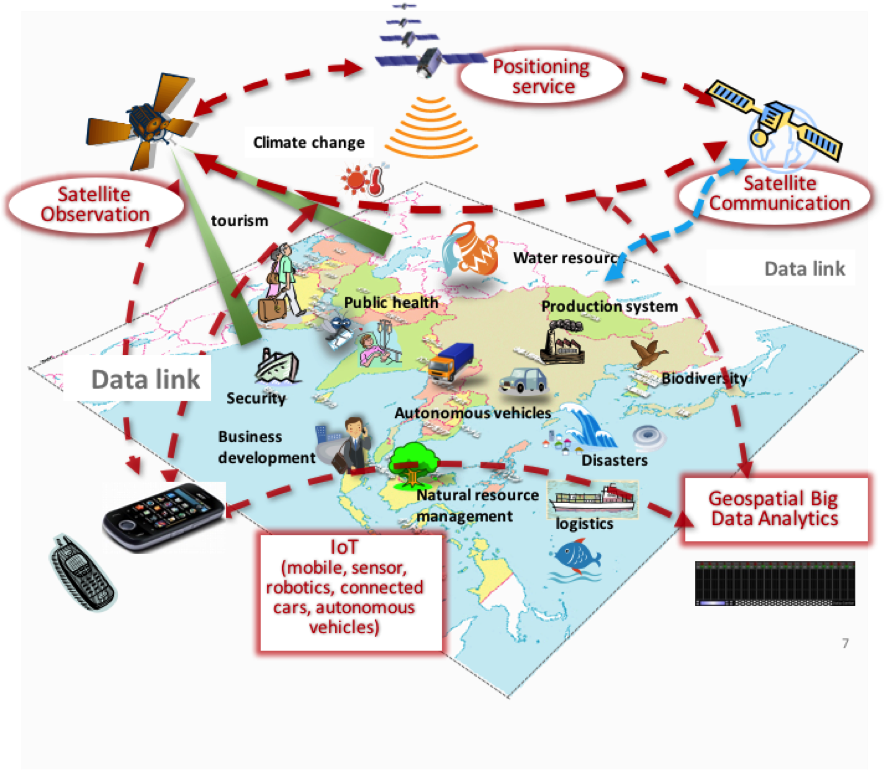
\includegraphics[width = 0.8\linewidth]{Figures/sgt.png}
\end{center}
\caption{Space infrastructure and technologies supporting SGT}
\label{sgt}
\end{figure}

SGT could provide diverse information services using “real-world data”. More concretely, in the context of the report, major services and contributions of SGT could be summarized as the following four aspects:

\begin{enumerate}

\item \textbf{Real-time localization and tracking} of people, cargo and vehicles (air, sea, and land).

\item \textbf{Real-time monitoring of environmental and contextual information} covering all land and sea, such as: dynamic maps (traffic, congestion, people flow, and city changes) or environmental changes (weather, water and air quality, and greenery) from which events, accidents, and disasters can be extracted. Silent but meaningful changes such as climate change and crustal deformation can be included.

\item \textbf{"Ubiquitous" data communications} at anytime/anywhere with small IoT devices to collect data from and to send instructions/guidance to people and machines in the field.

\item \textbf{High precision mapping} of 3D space and landscape framing activities of people and autonomous vehicles/machines, while it could include very slowly moving phenomena like crust movement monitoring.

\end{enumerate}


\vspace{0.4 cm}

\textbf{Satellite observation is extremely flexible and globally applicable} compared with airborne observation performed by aircraft or drones which suffers from airspace restriction, small coverage, and limited flight time. \textbf{Real-time positioning by satellites can be performed by compact and inexpensive portable terminals}, currently installed in almost all smart-phones as well as in most vehicles, airplanes, or ships. Therefore, the mobility data of people, vehicles, ships, and aircraft are widely available.

\vspace{0.4 cm}

Geostationary satellites are commonly used for data communication. However, the sufficient \textbf{miniaturization of ground transceivers combined with the use of the low earth orbit satellites constellation} will increase the access to efficient communication and dramatically reduce costs in a near future. Therefore, data communication services in other words, IoT-based data collection and dissemination will be available everywhere, as long as the sky is visible. 


\subsection{Generic examples of SGT application}

\tab Such a technological environment can be simultaneously established all over the world, allowing the promotion of a broad range of services in various countries and regions. 

For instance, small portable terminals equipped with Global Navigation Satellite Systems (GNSS) receivers are commonly distributed on land and sea, such as smart-phones, now widely distributed in most countries around the world. Also, the use of \textit{black boxes} --- a device combining a GNSS receiver with a wireless communication system, constantly transmitting its position --- in most ships and aircraft improved locational information collection of commercial vehicles. Finally, the development of IoT (Internet of Things) has allowed the collection and dissemination of data from various sensors scattered in fields.

As described earlier, the use of space infrastructure enables to understand the movement of individual persons, vehicles, and cargos. Furthermore, satellite imagery analysis helps visualize the background information or reasons behind people behavioral changes such as traffic congestion, disaster situations, construction of buildings and infrastructure, and changes of agricultural land.

\vspace{0.4 cm}

While the easy gathering of production-related information within factories has greatly contributed to the optimization of production processes, the collection of information related to external environment changes --- such as traffic jam, people flow, and disasters --- was hard to obtain. It is why optimization of industrial activities and production process is limited to inside of factories, not always covering the entire production system consisting of factory networks and logistics. SGT can help collecting this kind of information, in order to better understand the overall situations and facilitate tighter cooperation between various actors of the manufacturing and logistics sectors, leading to optimization of industrial activities in a broader scale. 

\vspace{0.4 cm}

Finally, for actors mostly involved in outdoor tasks such as construction, agriculture, fishery, and forestry, SGT allows to obtain very accurate locational and situational information for further optimization and automation.

\section{The various roles of SGT}

One of the original targets for the general civil application of SGT is disaster response. Based on an extensive number of previous studies and famous achievements in this field, it has been confirmed that SGT can be applied to the strengthening of the socioeconomic system and the development of efficient Disaster Risk Management (DRM) in the Association of Southeast Asia Nations (ASEAN).

\vspace{0.4 cm}

In this section, we first examine the use of the SGT in the field of DRM before discussing more generally the importance of data sharing in ASEAN countries.

\subsection{SGT for disaster management in ASEAN}

\tab The Asia-Pacific region, most populated region on Earth with more than 4.5 billion souls, is also the daily theater of the planet's deadliest disasters. 

The strong impacts of disasters in the Asia-Pacific region do not simply rely on the intensity of these unfortunate events but also on a set of systemic weaknesses of Asian countries: economic and financial fragility, galloping urbanization, exploding demography or lack of proper land use planning.

\vspace{0.4 cm}

One of the main reasons of the vulnerability of the Asia-Pacific region to disasters is its demography. Asia-Pacific is the most populated area in the world with more than 4.5 billion inhabitants in 2016 according to the United Nations Economic and Social Commission for Asia and the Pacific (UNESCAP) \cite{PopulationDataSheet}. In the region can be found most of the world's largest metropolises. In 2016, the United Nations estimated that 18 of the world's 31 megacities (more than 10 million inhabitants) were located in Asia-Pacific and that this number is expected to reach 24 out of 41 in 2030 \cite{WorldCities}. These high densities of population often located around riverside flood areas, along coastlines at risk of tsunami or at the base of landslide-prone mountains put large numbers of human life in jeopardy.

\vspace{0.4 cm}

In its 2015 Asia-Pacific Disaster Report, the UNESCAP dresses a sad portrait of the region. Between 2005 and 2014, 1,625 incidents had been reported. Most of these disasters were floods, followed, in order, by storms, earthquakes and tsunamis and landslides.

These disasters had a dramatic impact on the region's human security by killing almost half-million inhabitants in Asia-Pacific and were directly affecting the lives of approximately 1.4 billion people (see table \ref{HumanLossAP}). Moreover, beyond long term economic impact due to the loss of workforce as well as the increase of spending for health related issues, the 1,625 disasters evoked in the previous paragraph generated direct economic damages worth \$523 billion. 

\begin{table}[h]
   \caption{\label{HumanLossAP} Human impact of disasters in Asia and the Pacific, total 2005-2014 \cite{APdisaster2015}}
   \centering
   \begin{tabular}{| >{\columncolor[gray]{.9}}l | c | c |}
   \hline
     \rowcolor[gray]{.8}
     Disaster type & {Lives lost} & {People affected (millions)} \\
   \hline
    Earthquakes and tsunamis & 199,418 & 74 \\
    Storms & 166,762 & 321 \\
    Floods & 43,800 & 771 \\
    Others & 73,772 & 199 \\
   \hline  
    Total & 483,752 & 1,366 \\
   \hline   
   \end{tabular}
\end{table}

Finally, the UNESCAP report stresses the fact that although these numbers are impressive, they may be underestimated due to a lack of reliable  disaster data gathering initiative \cite{APdisaster2015}.

\vspace{0.4 cm}

Beyond natural disasters, strengthening food and water security is a priority for the development organizations operating in the region. According to an ADB report on food security, in 2010, more than 700 million people in Asia-Pacific survived with less than \$1.25 per day, in an environment where high and volatile food prices cause 537 million of them to suffer from hunger (62\% of the world) \cite{ADBfood}. Moreover, as 80\% of water resources are still exclusively used for agriculture, the region is particularly affected by water insecurity: 1.7 billion people do not have access to basic sanitation, 80\% of wastewater is directly dumped into rivers, lakes or seas with almost no treatment \cite{AWDO2016}. In terms of economic development, it is estimated that the annual global cost of water insecurity reaches \$500 billion, corresponding to a loss of more than 1\% global gross domestic product \cite{sadoff}. It goes without saying that the dramatic advance and intensification of climate change will considerably amplify all these issues as well as many others including water level increase, desertification, scarcity of available water resources, climate refugees/migrations or the intensification of large scale meteorological disasters. Finally, UNICEF recently raised an alarm about the increasing dangers posed by air-pollution. According to the UN agency's data, more than two billion children live in areas where outdoor air-pollution levels exceed WHO guidelines, including 1.07 billion in Asia-Pacific. Moreover, air pollution yearly kills 600,000 children under five years old.

\vspace{0.4 cm}

It is therefore primordial for ASEAN to develop and implement ambitious disaster risk management policies and strategy based on SGT. The following steps describes how SGT will contribute to the DRM via real-time tracking, monitoring, mapping and ubiquitous data communication capabilities:

\begin{itemize}
\item Monitoring and forecasting hazards at the local to regional scale, typically heavy rainfall, flooding, typhoon, drought and tsunami to let governments and people know what could happen.
\item Anticipating risks or damages on human lives and economic activities by overlaying the hazard prediction on the data of people distribution/activity information, vehicle movement and economic activity distribution/intensity.
\item Mitigating damages by guiding evacuation of people based on people distribution data and helping reconstruction of people lives and economic activities.
\item Improving preparedness by providing realistic simulations and trainings of DRM based on the historical records of disasters and reconstruction processes..
\end{itemize}

Steps above are made possible by sharing data among governmental agencies, private industries, NPOs and people. In this regards, SGT and more generally data sharing can play a prominent role, as clearly stated in the \textit{AADMER Work Programme 2016-2020} \cite{aadmer_wp}:

\begin{displayquote}

Promote regional standards, including methodologies and tools to assess, record, calculate the disaster losses and damages, and share non-sensitive data and create common information system, to enhance interoperability, ensure unity of action, and strengthen resilience.

\end{displayquote}

It should therefore be smartly and strongly designed, not only for disaster management but for multi-purpose usage, aiming at the strengthening of the regional  socioeconomic environment. Furthermore, beyond the impact of the system, it should be made in an economically sustainable way, which is a significant challenge.


\subsection{SGT for economic strengthening through enhanced connectivity} \label{enhanced}

As explained above, the potential of SGT incites users to go further than immediate issues like disaster by using it as an ambitious tool, at all level of the economy.

\vspace{0.4 cm}

SGT largely contributes to decision-making processes among governments, companies, communities, cities, individuals in various contexts by providing necessary information. As SGT enhances the economy and facilitates \textit{'smartification'} or \textit{'optimization'} across various kinds of "borders", such as a border between the inside and outside of a factory, borders among companies and regions/countries, it is extremely effective to connect all actors of ASEAN more tightly. Therefore, this study examines possible contributions of SGT system and data infrastructure to strengthen ASEAN connectivity.

\vspace{0.4 cm}

Furthermore, strengthening ASEAN connectivity is also essential for cross-border utilization of SGT. Therefore, the study also provides policy recommendations aiming at the enhancement of ASEAN connectivity, such as transboundary data transfer policy, in order to maximize the use of SGT.

\begin{figure}[H]
\begin{center}
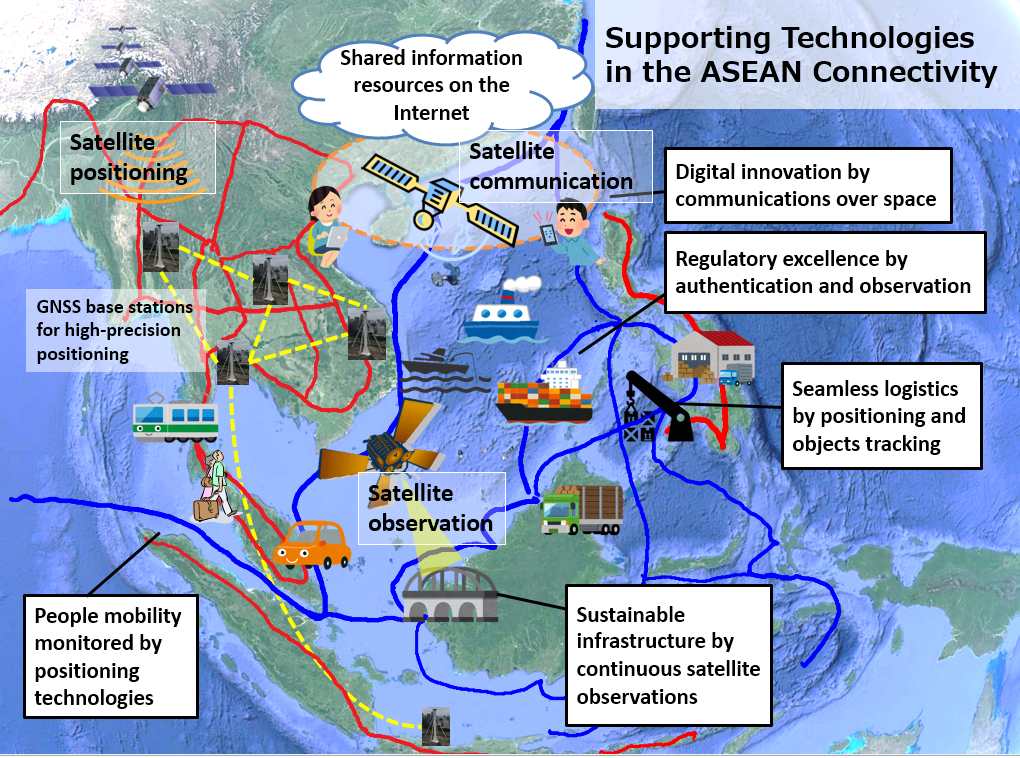
\includegraphics[width = 0.8\linewidth]{Figures/supp_connect.png}
\end{center}
\caption{Supporting technologies in the ASEAN connectivity}
\label{supp_connect}
\end{figure}

{\flushleft \bfseries Therefore, this study addresses:\par}
\vspace{0.2 cm}
{\bfseries A common platform and infrastructure of Space \& Geospatial Technology to enhance ASEAN connectivity and help realize human development, resiliency, and sustainable development. The sustainability of the system will reside in its value-creation process\par}

\vspace{0.4 cm}

The approach of this study is perfectly in line with the ambitious \textit{Master Plan on ASEAN Connectivity 2025} or \textit{MPAC-2025} \cite{mpac}. Adopted in 2016, it targets the following sectors as main contributors to ASEAN Connectivity Strategies: Sustainable Infrastructure, Digital Innovation, Seamless Logistics, Regulatory Excellency, and People Mobility. SGT can contribute to these strategies, by being advantageously utilized for addressing common issues, developing common interests, and creating common infrastructures.

\vspace{0.4 cm}

In addition, SGT is expected, in the \textit{ASEAN Socio-Cultural Community Blueprint 2025} (ASCCB-2025) \cite{asccb}, to contribute to make ASEAN more:

\begin{itemize}
\item \textbf{Sustainable} through its application on biodiversity conservation, climate change, urbanization, production, and consumption.
\item \textbf{Resilient} through disaster response and health care. 
\item \textbf{Dynamic} through science and technology development.
\end{itemize}

These strategies and solutions can be efficiently expanded to the entire ASEAN region thanks to the extensiveness, the immediacy and the transboundary nature of space technologies.

\vspace{0.4 cm}

Specifically, while levels of ground infrastructure maintenance greatly vary with the degree of economic development, space system can provide the same information and services to the whole region. Therefore, strategies and good practices obtained from the MPAC-2025 and the ASCCB-2025 can be freely applied to ASEAN countries by overcoming national infrastructural limitations.


\section{Towards a data-driven ASEAN}

\tab At the end of 2015, the OECD published a major report entitled \textit{Data-Driven Innovation -- Big Data for Growth and Well-Being}. It states that \textit{'digitalization'} and data conversion of various activities will be advanced innovations, and a new economy will be developed accordingly \cite{oecd_ddi}.

The existing various common infrastructures (communication and meteorological satellites) and traditionally dynamic interactions (trade, information sharing, and interaction) in the ASEAN region makes the ASEAN the perfect place for the emergence of upgraded version of data-driven innovation economy (DDIE). In particular, by removing physical restrictions, SGT will support ASEAN transformation into a DDIE 2.0.

\begin{figure}[H]
\begin{center}
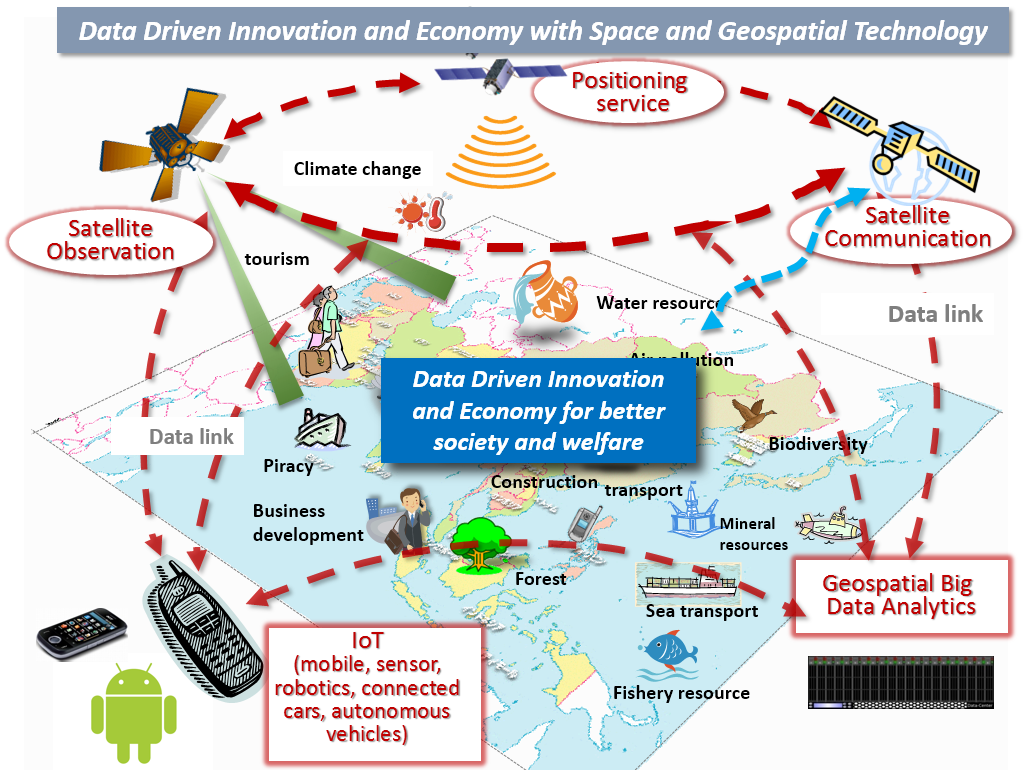
\includegraphics[width = 0.8\linewidth]{Figures/data_driven.png}
\end{center}
\caption{Data driven society through SGT}
\label{data_driven}
\end{figure}

\subsection{The tremendous economic potential of SGT}

\tab To understand more the prominent role that could be played by SGT in promoting innovation in ASEAN, let us look again at the MPAC-2025 \cite{mpac}. In its focus on digital innovation, it claims that:

\begin{displayquote}

Disruptive technologies (particularly mobile Internet, big data, cloud technology, the Internet of Things, the automation of knowledge work and the Social-Mobile-Analytics-Cloud or SMAC) could unleash some \$220 billion to \$625 billion in annual economic impact in ASEAN by 2030.

\end{displayquote}

In other words, it is SGT that will help to unleash these hundreds of billion USD, which may be derived from increased efficiency, new products and services, etc.

\subsection{From local to global optimization} \label{optimization}

As briefly explained above, one of the greatest strengths of SGT is its capacity to go beyond local optimization --- at factory level --- to achieve global optimization --- taking into account dynamically changing external factors and interrelations.

\vspace{0.4 cm}

The use of digital technology for monitoring and control within factories is already well developed, allowing an optimal use of resources and means of production for the production system in a factory.

However, information sharing such as logistics between the factory and its partners (distributing networks, providers, etc.) is very insufficient. Any logistical irregularity will impact the whole production system, independently from the quality of the local optimization within the factory.

\begin{figure}[H]
\begin{center}
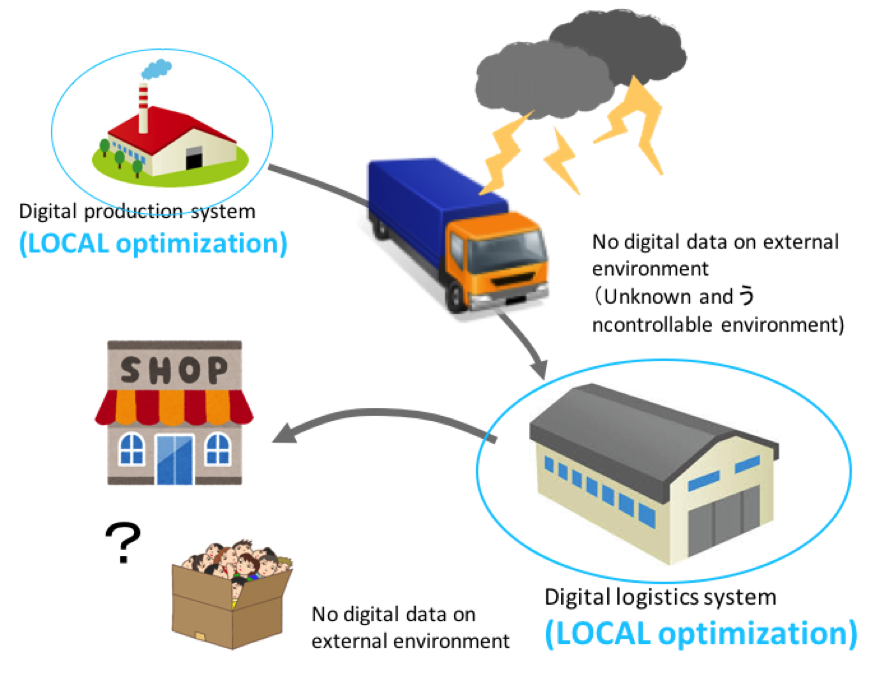
\includegraphics[width = 0.7\linewidth]{Figures/local_optimization.png}
\end{center}
\caption{Local optimization}
\label{local_optimization}
\end{figure}

Therefore, changes in the external environment can be major risks when data cannot be obtained, showing the limits of local optimization, as described on figure \ref{local_optimization}. While external environment cannot be directly controlled, if real-time data can be obtained, the production system can be adapted to the changes and risks can be significantly reduced.

Furthermore, in sector organized around outdoor activities, such as in construction, agriculture, forestry and fishery industries, sufficient information required for the production cannot be easily obtained. 

\vspace{0.4 cm}

SGT seamlessly digitalizes all spaces including external environments. It is therefore possible to optimize the entire system by considering external environmental changes. Figure \ref{global_optimization} expresses this idea.

\begin{figure}[H]
\begin{center}
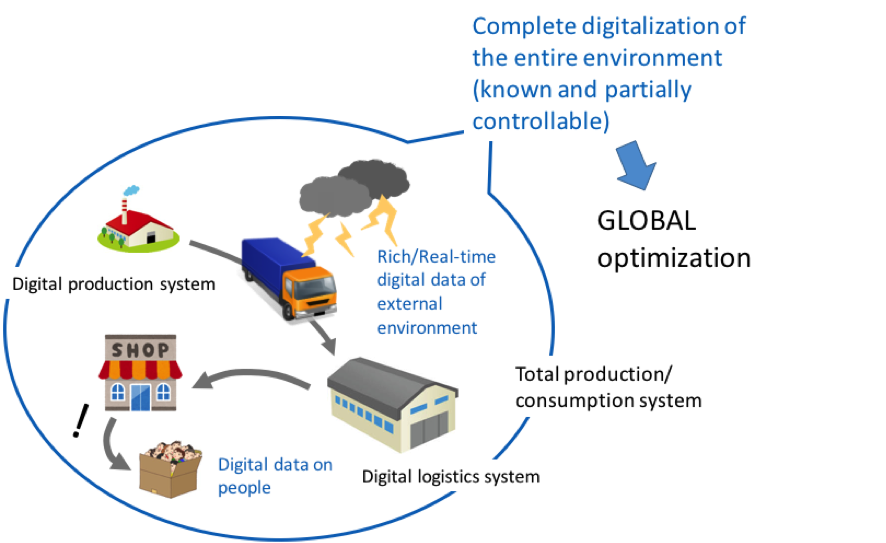
\includegraphics[width = 0.8\linewidth]{Figures/global_optimization.png}
\end{center}
\caption{Global optimization}
\label{global_optimization}
\end{figure}


\subsection{Achieving the third unbundling} \label{unbundling_p}

\tab In the current ASEAN situation, without widespread SGT applications, the optimization process of the whole production system connecting companies is extremely complicated as external environment is largely unknown. As a result, companies try to optimize their own production as much as possible by incorporating them into a single organization (e.g. factory) all productive actors, hence, drastically reducing unbundling. Figure \ref{unbundling} shows the concept of unbundling in production and industrial systems.

\begin{figure}[H]
\begin{center}
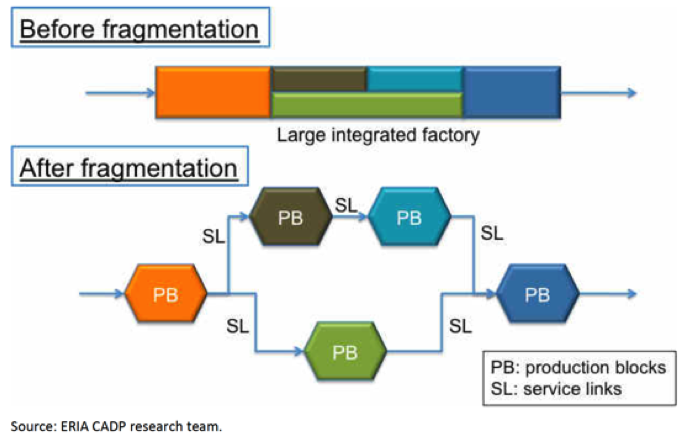
\includegraphics[width = 0.8\linewidth]{Figures/unbundling.png}
\end{center}
\caption{The concept of unbundling}
\label{unbundling}
\end{figure}

However, if sufficient digital data on external environment are obtained, it is possible to control the whole production system for optimization by incorporating the external changes. As a result, it is not required to build up each component of a production system in the company. Unbundling of the production system can be advanced to a large scale.

\vspace{0.4 cm}

While a change in logistics thanks to SGT accelerates the 2nd unbundling --- spatial separation of production blocks, it is expected that the spatial separation of engineers and managers involved in the production will also be further accelerated. This \textbf{3rd unbundling} will be achieved through the digitalization of production systems that is to say the digitalization of people, goods, and real-time monitoring.


\subsection{Conclusion: Enhancing ASEAN digitalization and connectivity with SGT}

In summary, Data Driven Innovation as proposed by the OECD is a general concept stating that industrial innovation will be developed through data utilization.

On the other hand, SGT effectively facilitates the optimization of the whole economic system --- production, consumption, services, etc. --- by digitalizing the external environment of individual production and business activities. 

\vspace{0.4 cm}

In ASEAN, where sudden external environmental changes, such as disasters, frequently occur, DDIE associated with SGT plays a significant role. Understanding such changes is not only important for the optimization of production systems but is also essential for improving social welfare including life stability and safety of local populations.

It can therefore be said that SGT will rapidly strengthen the inter-connectivity of ASEAN countries. As a result, it will strongly support industrial innovation, economic advancement, and social welfare.

\vspace{0.4 cm}

{\bfseries In short, Space \& Geospatial Technologies will create immense value through the realization of Data-Driven Innovation and Economy 2.0 and the Third Unbundling in ASEAN.}





















